\section{Результаты работы пятой лабораторной работы}

\subsection{Задание 1}

Используя таблицу освоенного объема, определите основные
финансовые показатели проекта на указанную дату отчета.

Вид => Таблицы => Другие таблицы:

\begin{figure}[ht!]
	
\includegraphics[width=0.75\linewidth]{assets/images/volume.png}
	\label{fig:r2}
	\caption{Таблица основного объема}
\end{figure}
\FloatBarrier

\begin{figure}[ht!]
	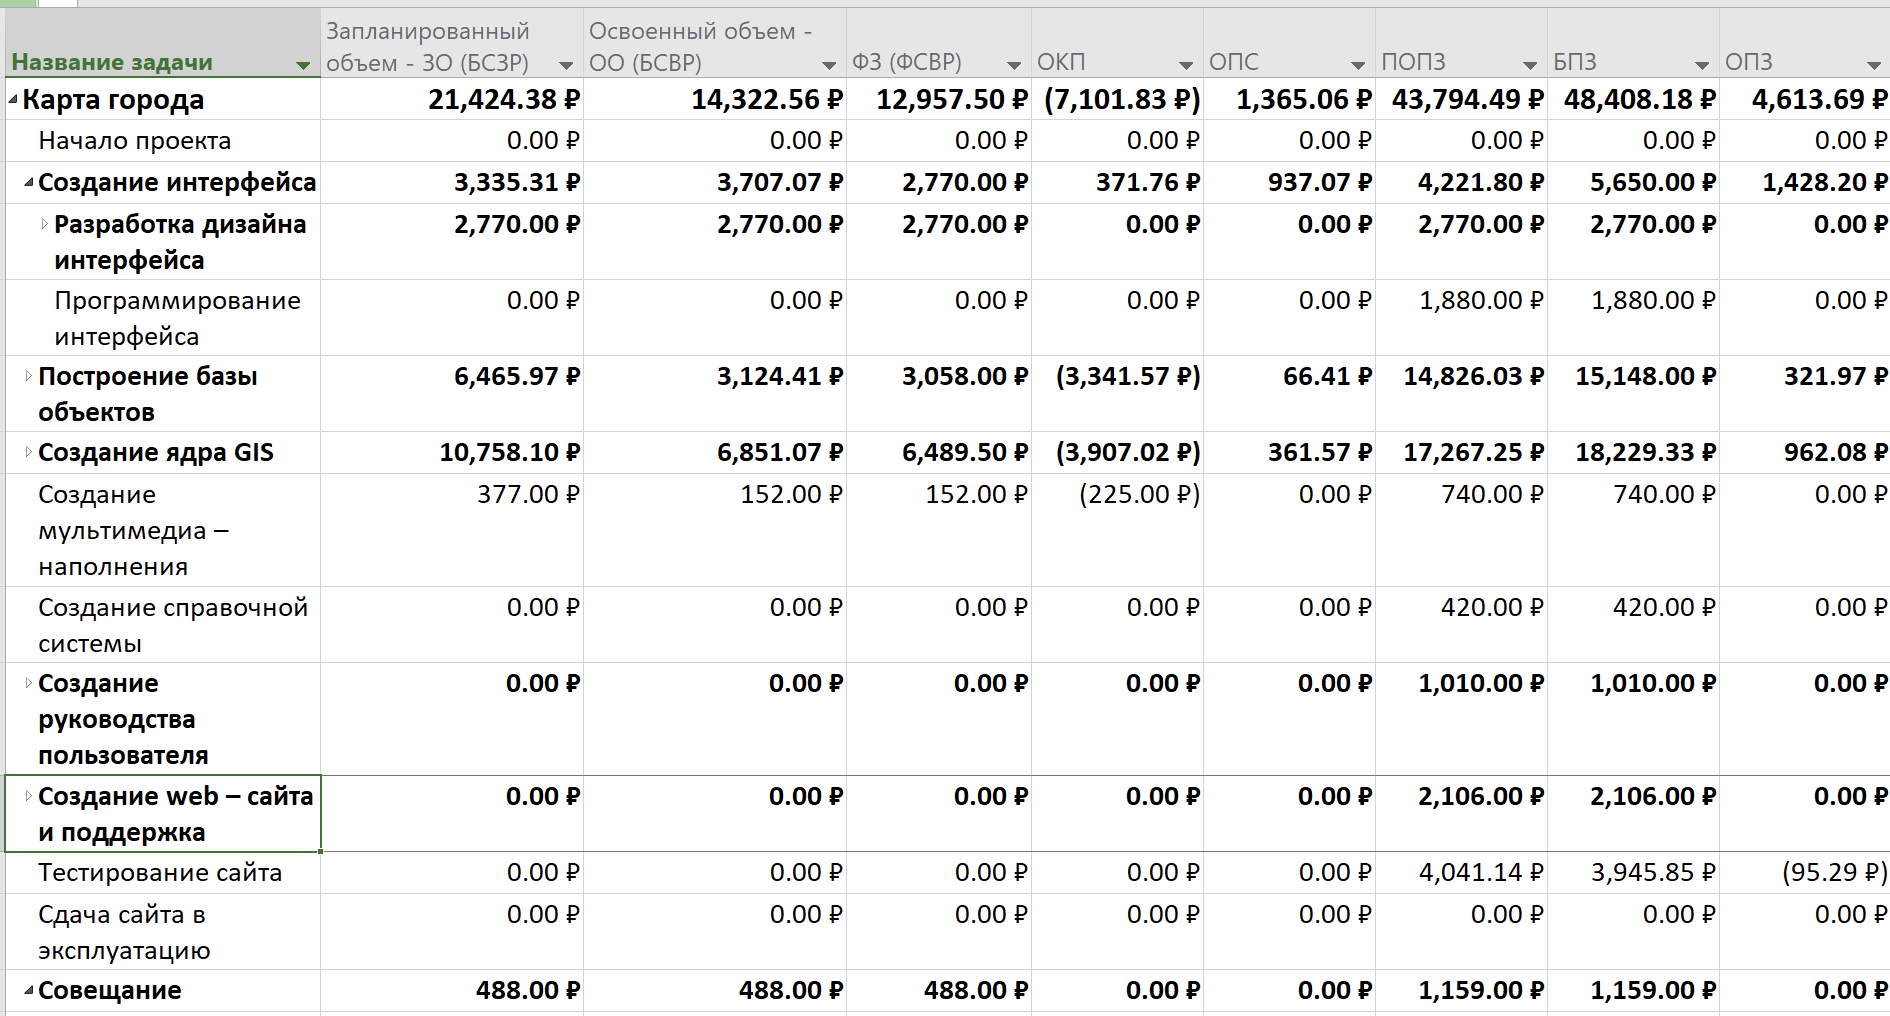
\includegraphics[width=0.75\linewidth]{assets/images/new-gant.png}
	\label{fig:r2}
	\caption{Финансовые показатели}
\end{figure}
\FloatBarrier

Основные финансовые показатели:
1. Запланированный объем (ЗО) – это средства, которые были затрачены
на выполнение задачи в период с начала проекта до выбранной даты
отчета, если бы задача точно соответствовала графику и смете.

2. Освоенный объем (ОО) – это средства, которые были бы затрачены на
выполнение задачи с самого начала проекта до выбранной даты отчета,
если бы фактически выполненная работа оплачивалась согласно смете,
т.е. это фактическое количество рабочих часов, оплачиваемых по
сметным ставкам.

3. Фактические затраты (ФЗ) – средства, фактически потраченные на
задачи в период с начала проекта до выбранной даты отчета.

4. Отклонение от календарного плана (ОКП) позволяет вычислить
несоответствие сметы, которое вызвано различием между плановым и
фактическим объёмом работы, если это величина меньше 0, то проект
опаздывает.

5. Отклонение по стоимости (ОПС) сравнивает сметную и фактическую
стоимость выполненной работы и позволяет выделить несоответствие
сметы, вызванные разницей стоимости ресурсов, если эта величина
меньше нуля, то проект вышел за пределы сметы.

6. Предварительная оценка по завершении (ПОПЗ) отображает
ожидаемые общие затраты для задачи, расчет которых основан на
предположении, что оставшаяся часть работы будет выполнена в точном
соответствии со сметой. (прогноз по завершении)

7. Затраты по базовому плану (БПЗ) показывают фиксированные
затраты и стоимость ресурсов согласно базовому плану.

8. Отклонение по завершению (ОПЗ) – разность между БПЗ и ПОПЗ,
если эта величина отрицательна, то наблюдается перерасход средств.

Результат на скрине ниже. По нему видно, что на момент отчета освоенный
объём (14 322,56) меньше запланированного (21 424,38). Совещания в
точности соответствуют плану. А вот задача создания интерфейса превышает
на 470,06 рублей. То же самое можно сказать про построение базы объектов,
только разница составляет несколько тысяч.
Что касается задачи создания мультимедиа-наполнения, то наблюдается
обратная картина: освоенный объем меньше запланированного (на 220 рублей).
Если рассматривать весь объект в целом, то освоенный объем меньше на
7102,18 рублей, чем запланированный объем.

10 Задача отклонился от бюджета, так как программист 3 заболел.
И поэтому задача стала выполнятсья дольше, и за счет этого затраты на нее увеличились.
Также повлияло, то что задача считается выполнена на 80 процентов.

11 Задача наполнение базы объектов также отошла от базового плана, так как сроки предыдущей задачи сместились.

13 Задача анализ и проектирование ядра увеличись, так как сисетмный аналитик стал работать на полставки.

И задачи следующий отклонились по бюджету, так как сроки 10 задачи сдвинулись.

Таким образом, на 29.04.2022:

1. Затраты по базовому плану (БПЗ) –-- 48 408,18 рублей

2. Отклонения от базового плана:

a. Отклонение от календарного плана (ОКП) < 0, проект не опережает
план

b. Отклонение по стоимости (ОПС) > 0, проект находится в пределах
сметы, наблюдается экономия средств (1365.06 рублей)

c. Отклонение по завершению (ОПЗ) > 0, нет перерасхода средств,
проект укладывается в смету (4613.69)

\subsection{Задание 2 Работа с отчетами проекта}

1. Определите, в какой период времени руководитель проекта будет
испытывать наибольшую потребность в деньгах.

2. Выведите на экран задачи, превышающие бюджетную стоимость.

3. Определите задание для ресурса, указанного преподавателем.

Отчет => Наглядные отчеты => Отчет о бюджетной стоимости.

\begin{figure}[ht!]
	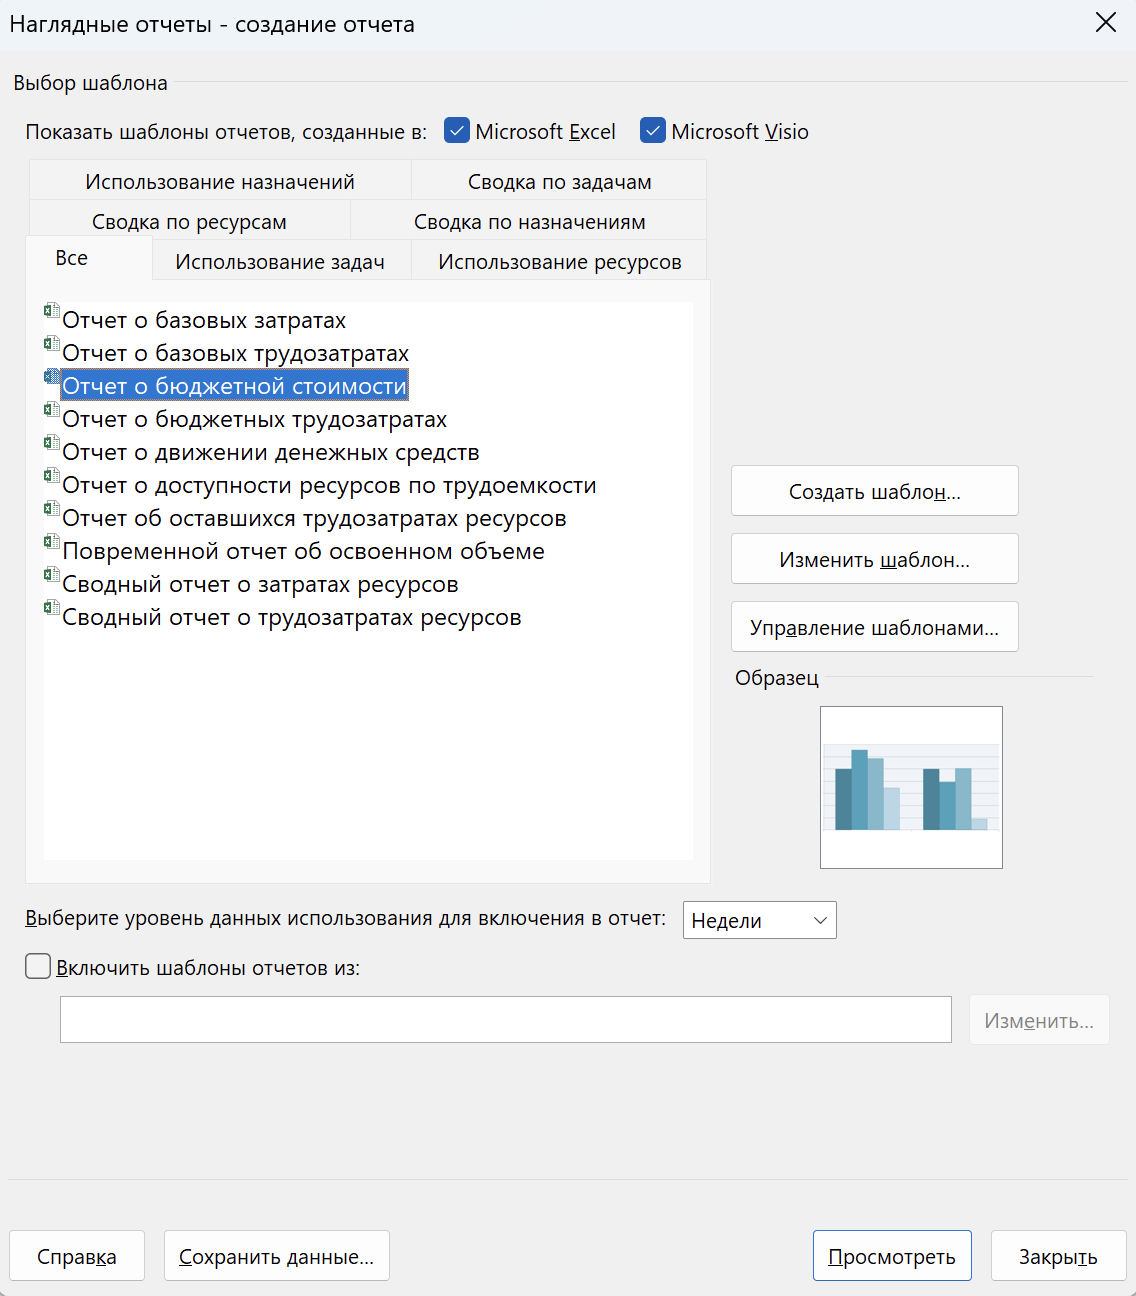
\includegraphics[width=0.75\linewidth]{assets/images/Отчет о бюджетной стоимости.png}
	\label{fig:r2}
	\caption{Отчет о бюджетной стоимости}
\end{figure}
\FloatBarrier

\begin{figure}[ht!]
	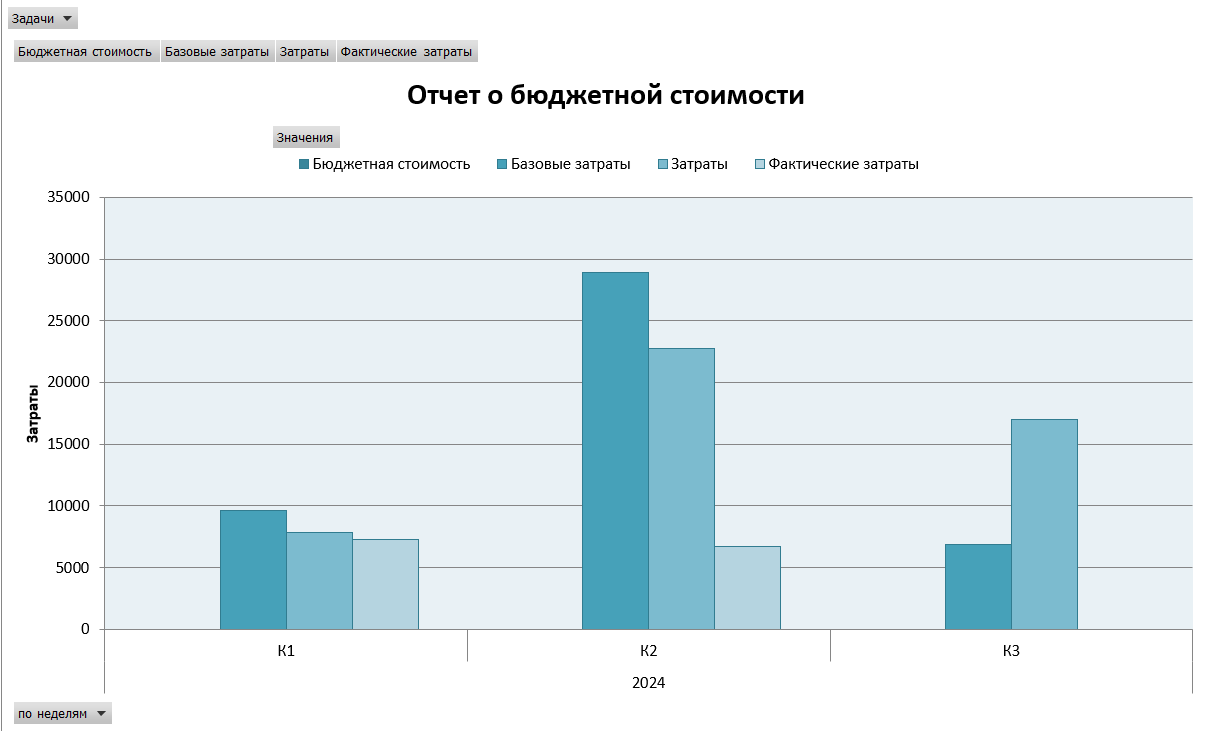
\includegraphics[width=0.75\linewidth]{assets/images/image_2024-03-16_09-06-31.png}
	\label{fig:r2}
	\caption{Отчет о бюджетной стоимости}
\end{figure}
\FloatBarrier

\begin{figure}[ht!]
	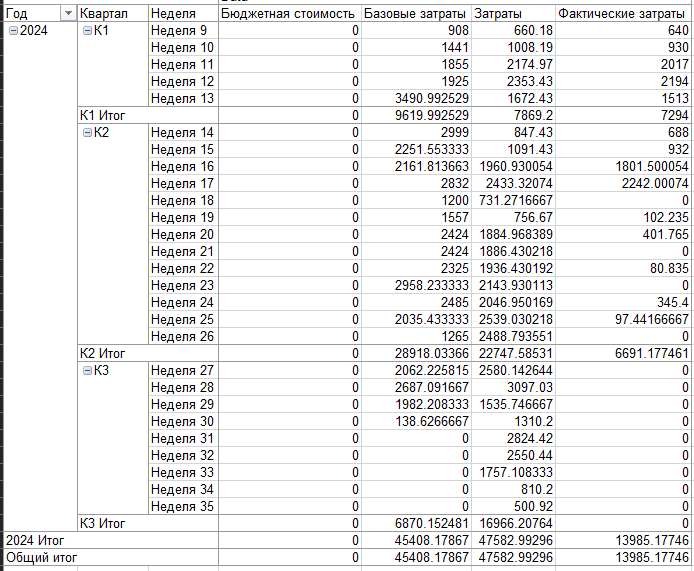
\includegraphics[width=0.75\linewidth]{assets/images/image_2024-03-16_09-10-00.png}
	\label{fig:r2}
	\caption{Отчет о бюджетной стоимости}
\end{figure}
\FloatBarrier

\begin{figure}[ht!]
	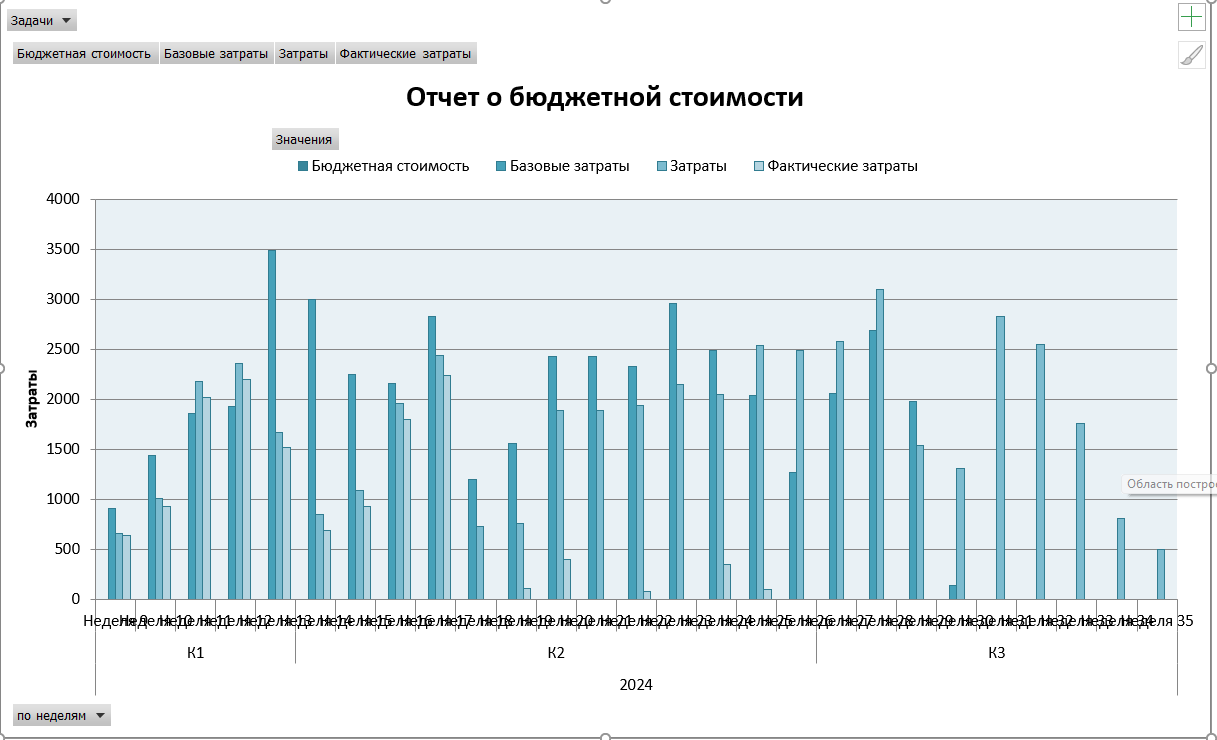
\includegraphics[width=0.75\linewidth]{assets/images/image_2024-03-16_09-10-56.png}
	\label{fig:r2}
	\caption{Отчет о бюджетной стоимости}
\end{figure}
\FloatBarrier

Наибольшая потребность в деньгах руководитель проекта будет испытывать
на 12, 22 и 27.

На 12 неделе начинаются такие задачи как: Анализ и проектирование, Разработка 2D и 3D.

На 22 –-- Создание модели ядра, Анализ и построение структуры БД, создание
заставки, Построение базы объектов, к тому же, на эту неделю выпадает
покупка своего сервера.

На 27 --– Создание рабочей модели, Программирование интерфейса, Разработка
дизайна, Написание руководства пользователя, Наполнение базы объектов.

\begin{figure}[ht!]
	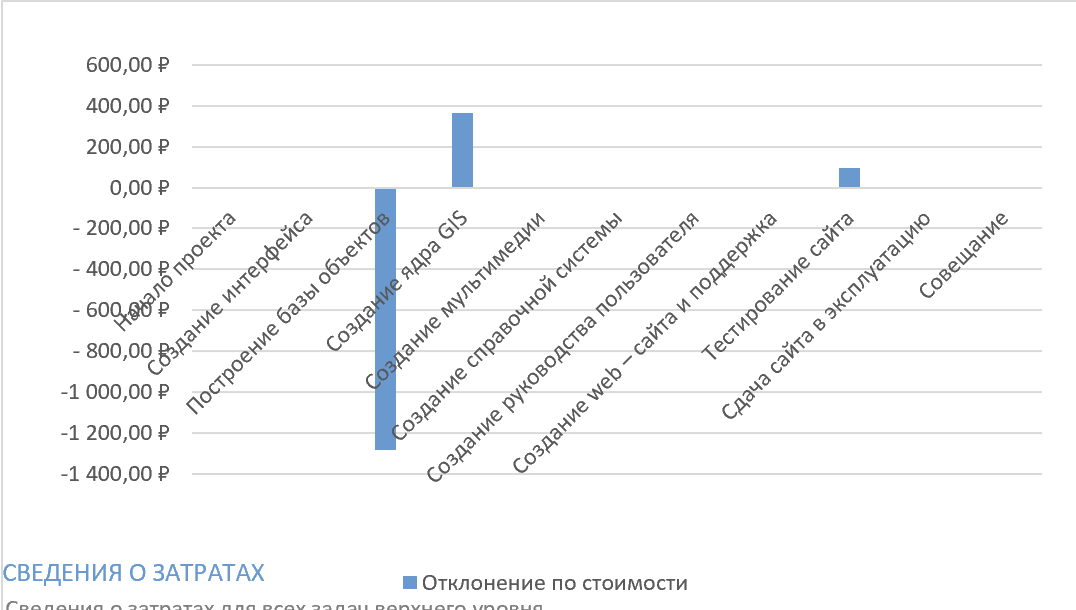
\includegraphics[width=0.75\linewidth]{assets/images/Screenshot 2024-03-16 at 12.57.15.png}
	\label{fig:r2}
	\caption{Отклонение по стоимости задачи}
\end{figure}
\FloatBarrier

Основное отклонение у построение базы объектов.

\begin{figure}[ht!]
	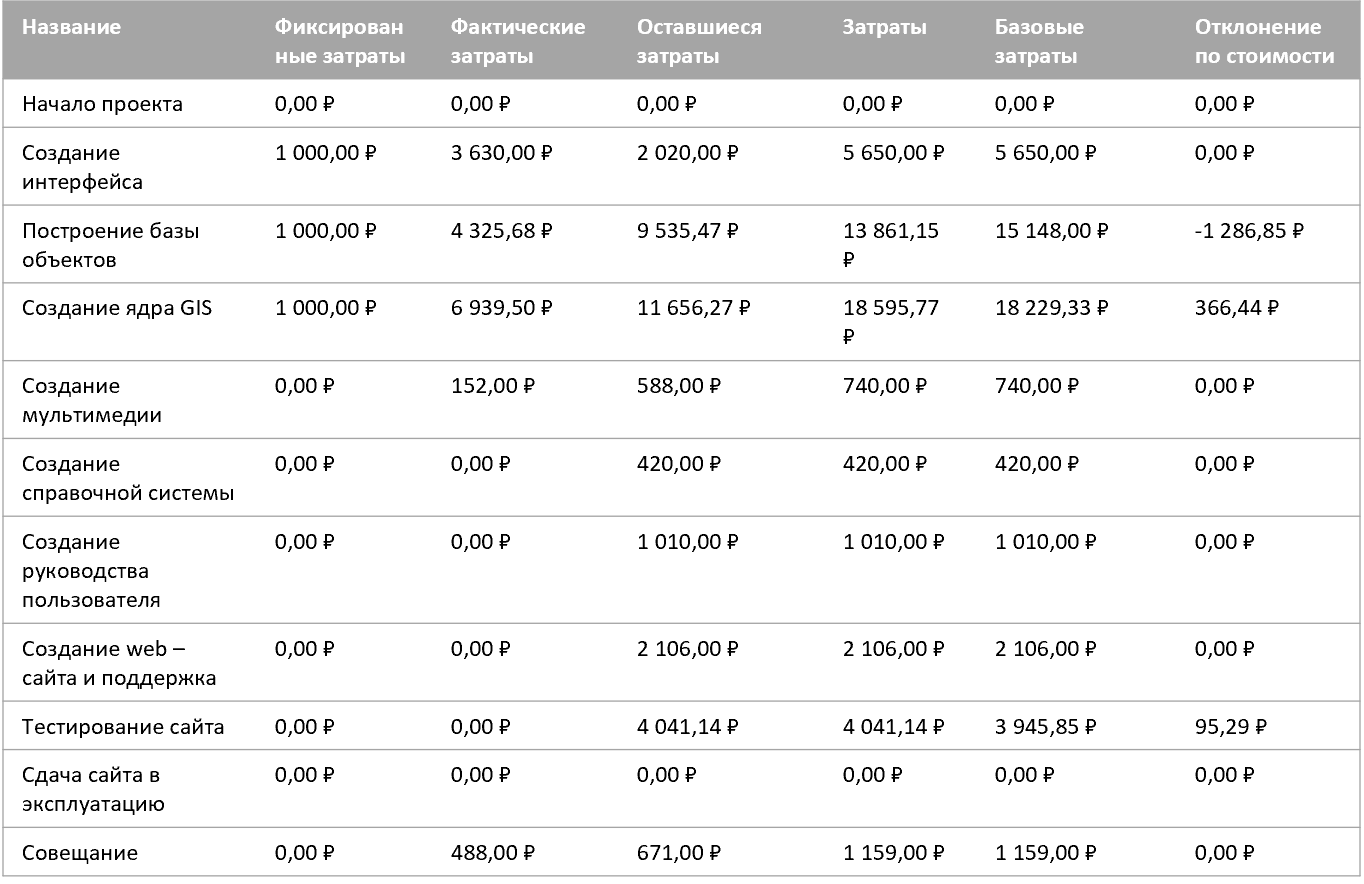
\includegraphics[width=0.75\linewidth]{assets/images/Screenshot 2024-03-16 at 12.58.51.png}
	\label{fig:r2}
	\caption{Отклонение по стоимости задачи}
\end{figure}
\FloatBarrier

\begin{figure}[ht!]
	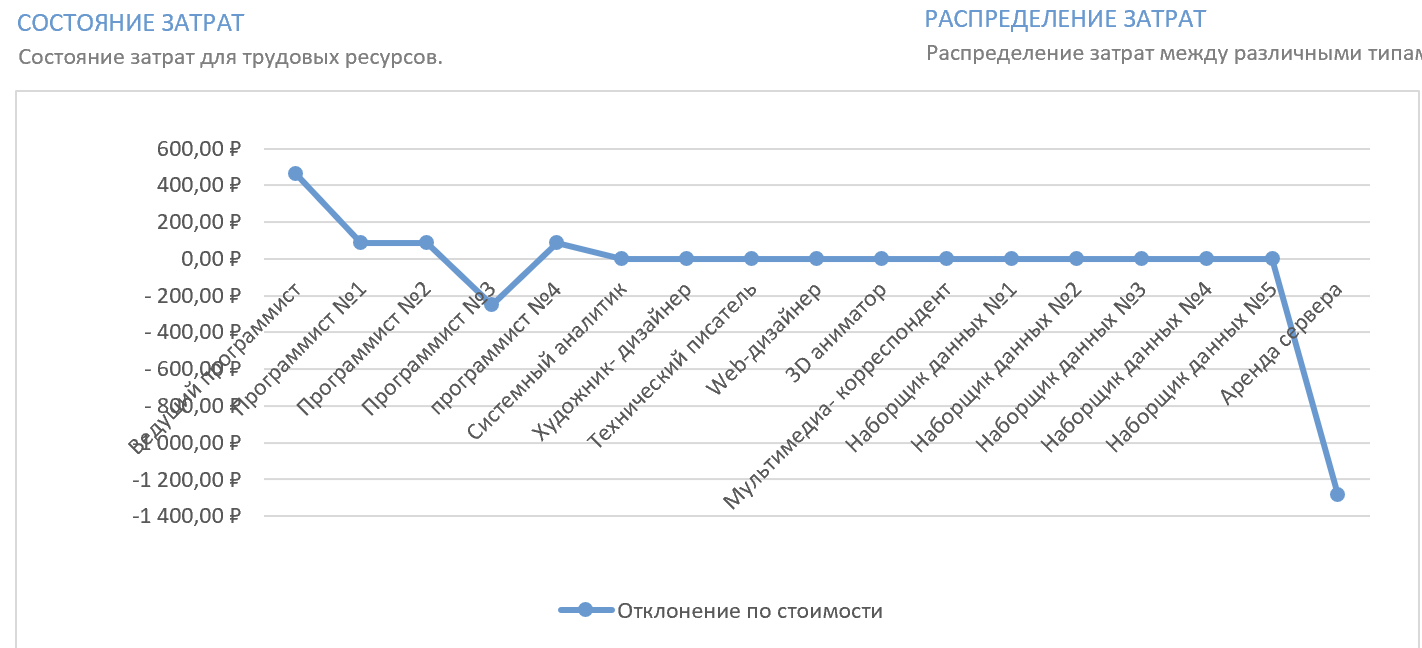
\includegraphics[width=0.75\linewidth]{assets/images/Screenshot 2024-03-16 at 12.59.47.png}
	\label{fig:r2}
	\caption{Отклонение по стоимости рессурсов}
\end{figure}
\FloatBarrier

Такие показатели из-за увелечения стоимости сервера и из-за того, что заболел программист 3, и повышение квалификации у ведущего программиста.

\begin{figure}[ht!]
	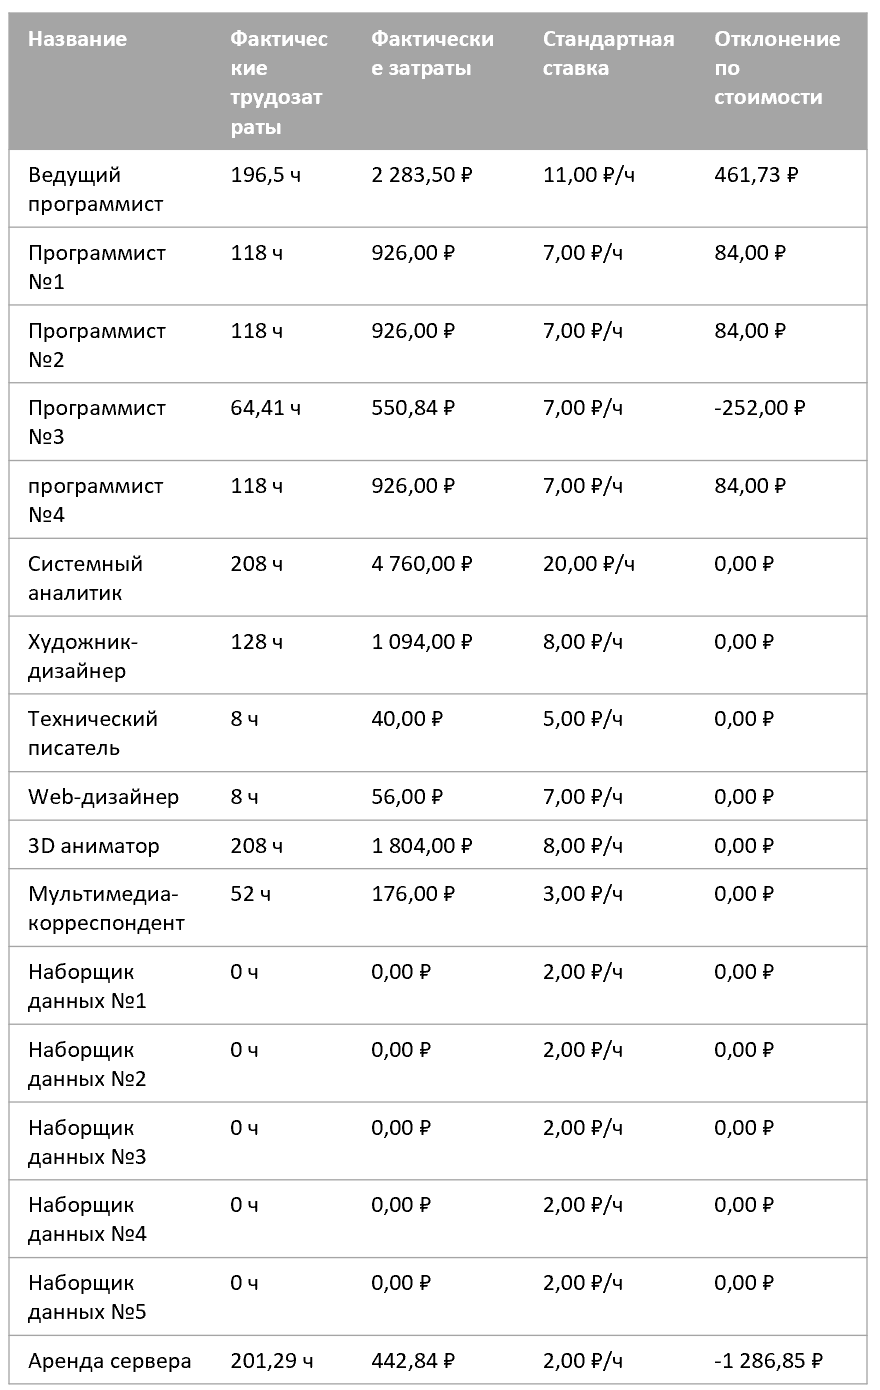
\includegraphics[width=0.75\linewidth]{assets/images/Screenshot 2024-03-16 at 13.02.19.png}
	\label{fig:r2}
	\caption{Отклонение по стоимости рессурсов}
\end{figure}
\FloatBarrier

\subsection{Задание 3: Анализ вариантов декомпозиции работ в проекте}

1. Предложите другой вариант декомпозиции работ, сохранив
длительности элементарных задач и первоначально выделенные для их
выполнения ресурсы. Оцените параметры проекта, устранив перегрузку
ресурсов и оптимизировав критический путь проекта.

2. Сделайте выводы о преимуществах и недостатках каждого из вариантов
планирования, которые отразите в отчете.

До:

\begin{figure}[ht!]
	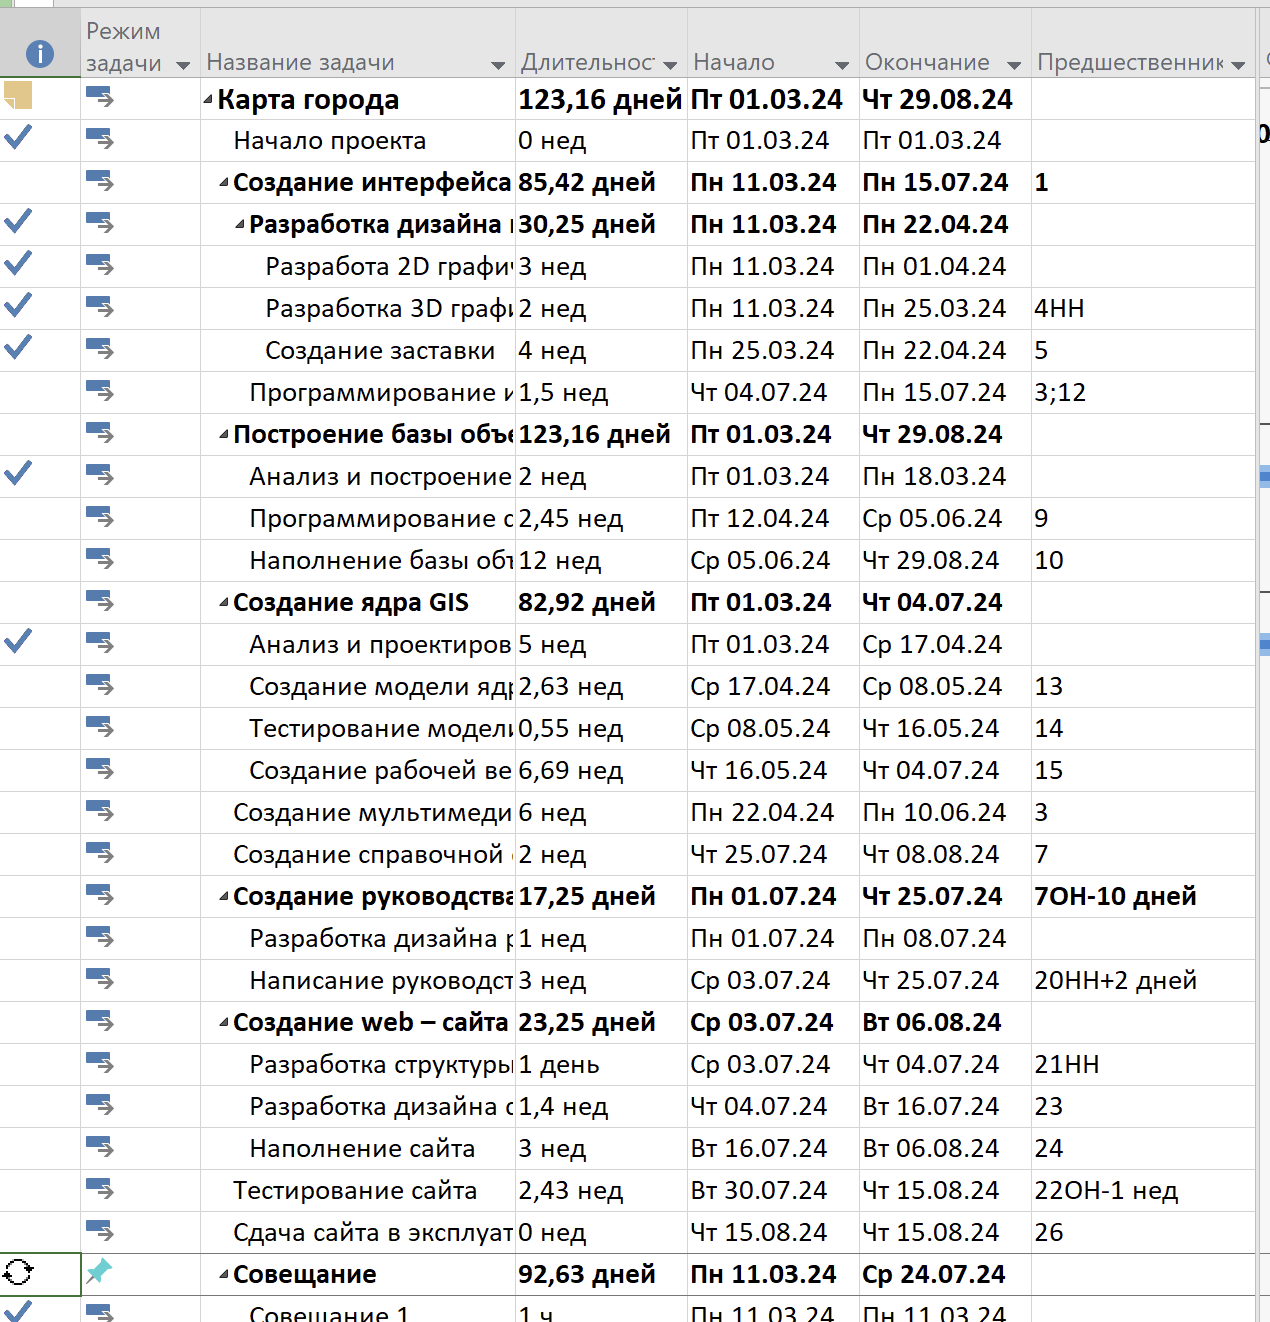
\includegraphics[width=0.75\linewidth]{assets/images/Screenshot 2024-03-16 at 13.16.44.png}
	\label{fig:r2}
	\caption{До}
\end{figure}
\FloatBarrier

\begin{figure}[ht!]
	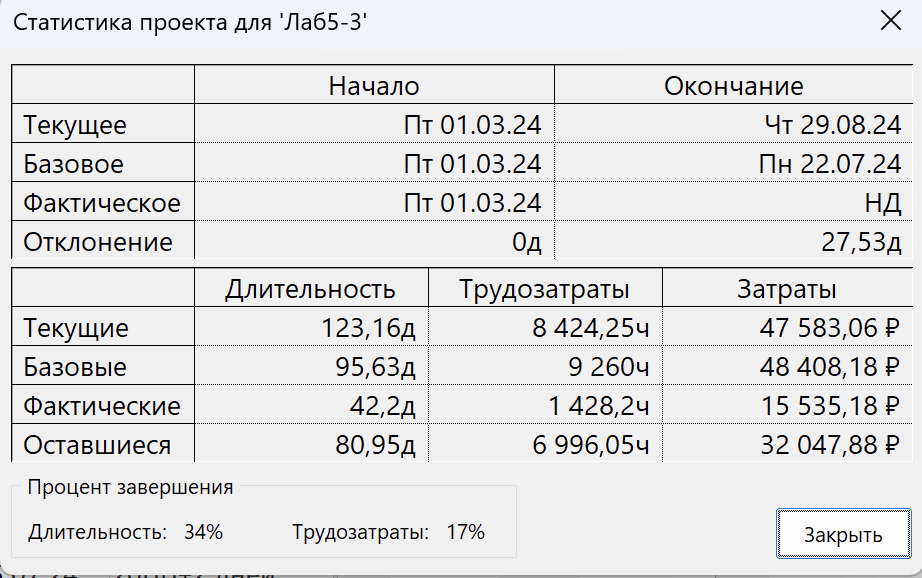
\includegraphics[width=0.75\linewidth]{assets/images/Screenshot 2024-03-16 at 13.17.33.png}
	\label{fig:r2}
	\caption{До}
\end{figure}

После:

Была проведена декомпозиция по процессам –-- анализ и проектирование,
разработка, программирование, заполнение данными.
В результате срок завершения не сместился, а что касается затрат, то они уменьшились примерно на 2000.

\begin{figure}[ht!]
	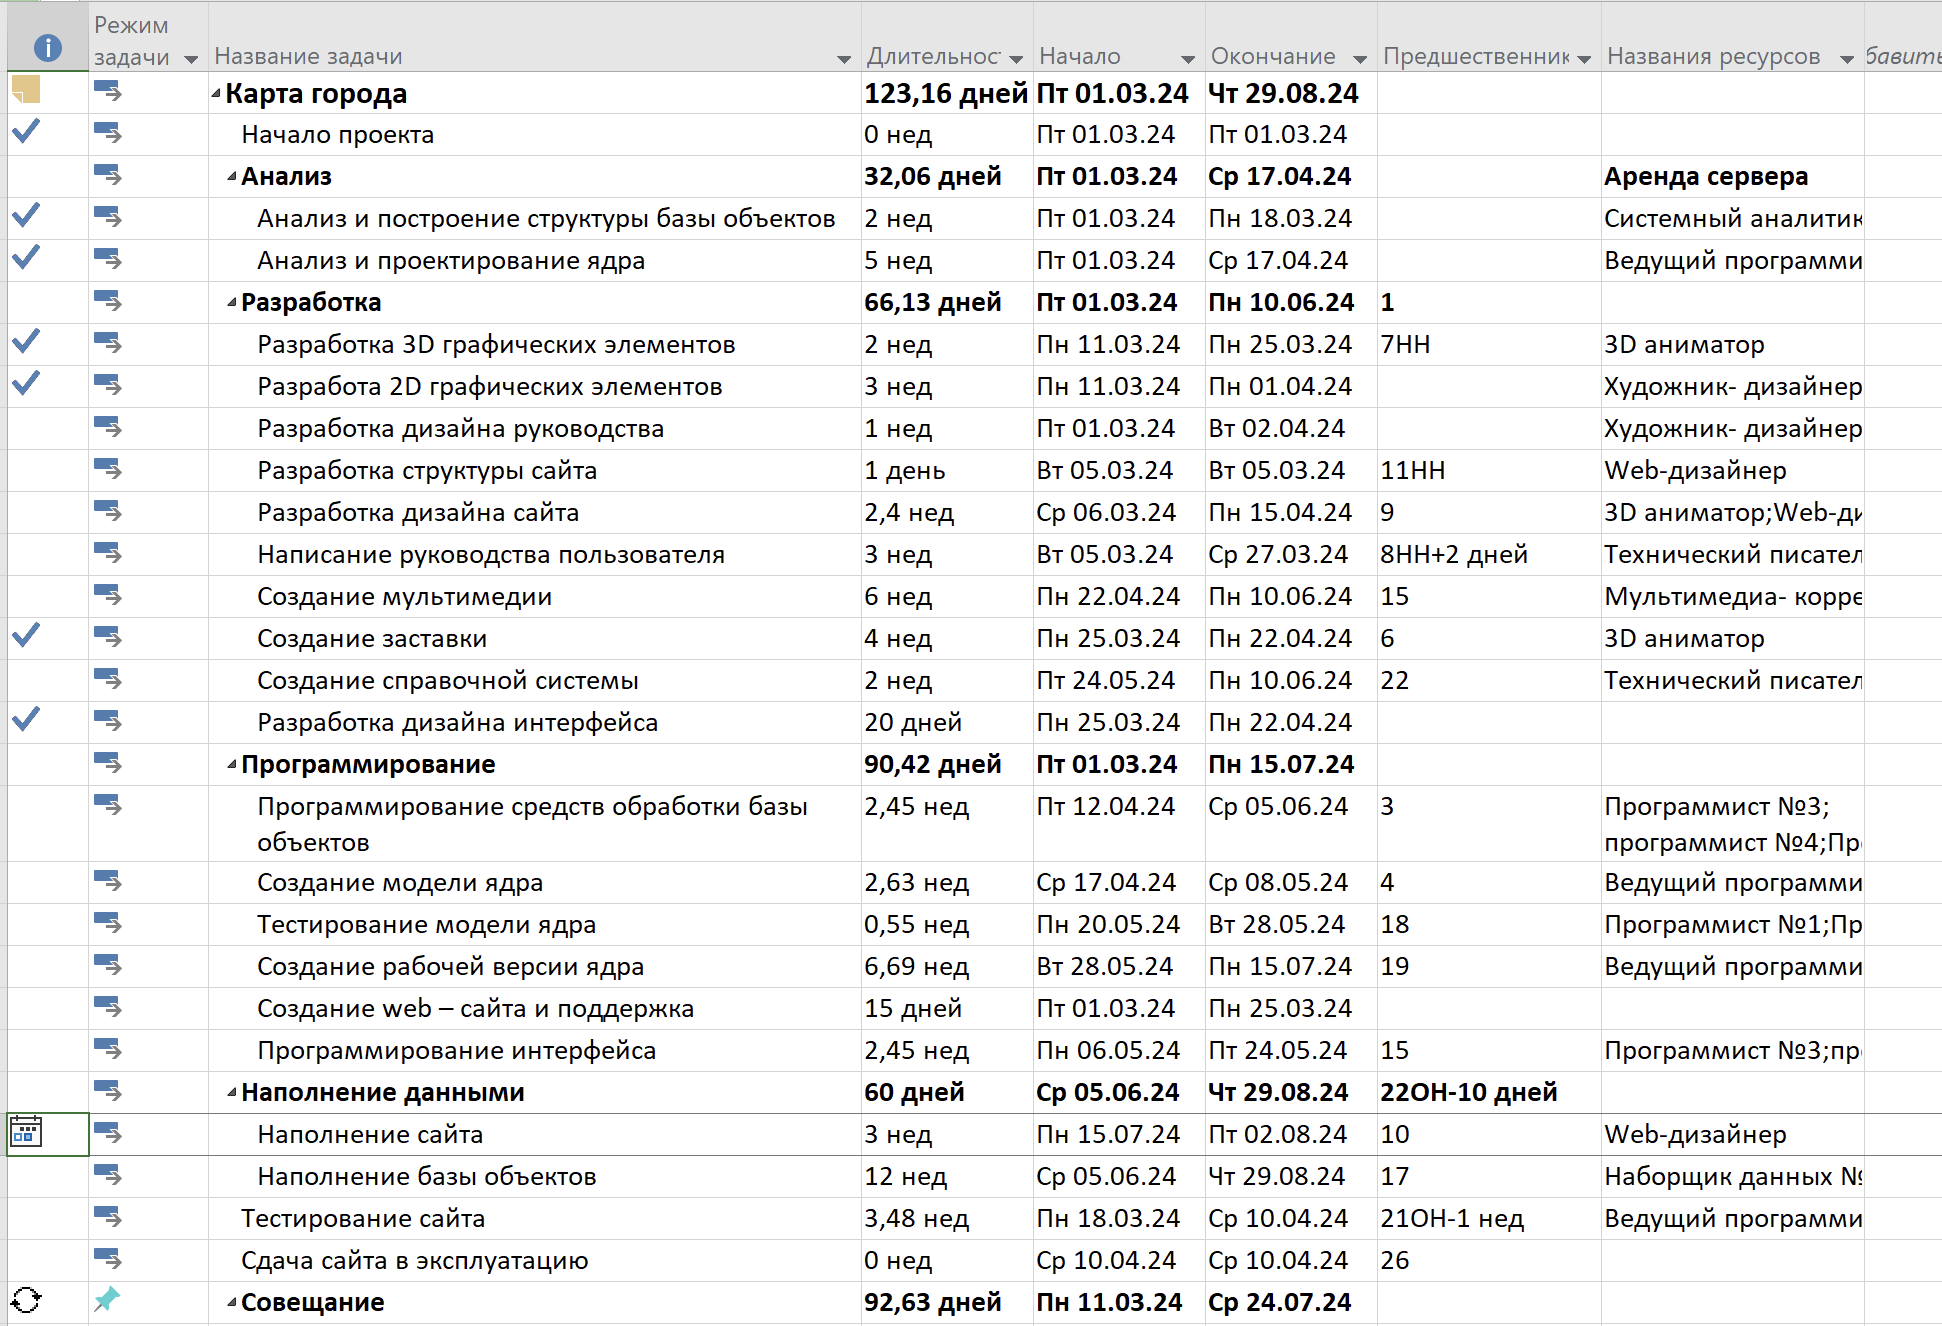
\includegraphics[width=0.75\linewidth]{assets/images/Screenshot 2024-03-16 at 13.57.35.png}
	\label{fig:r2}
	\caption{После}
\end{figure}
\FloatBarrier

\begin{figure}[ht!]
	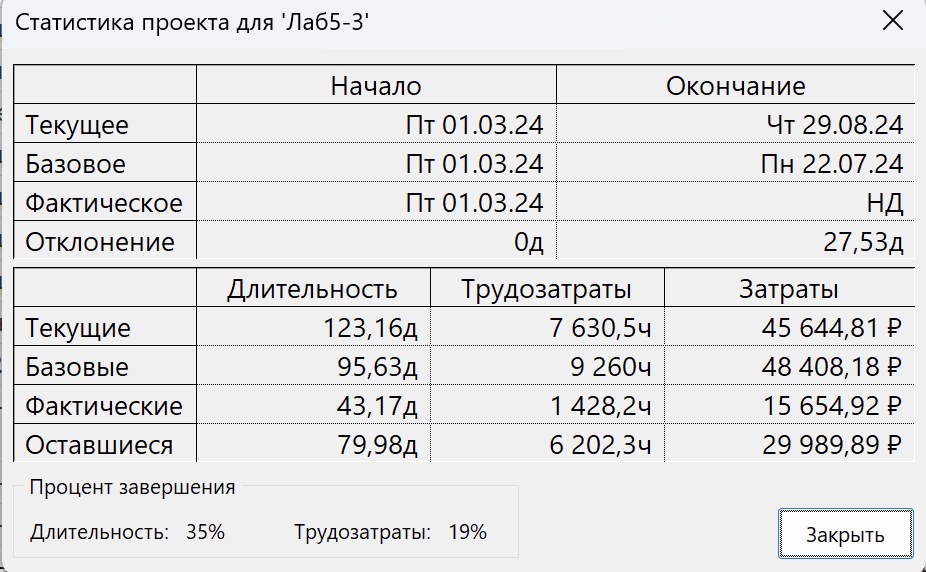
\includegraphics[width=0.75\linewidth]{assets/images/Screenshot 2024-03-16 at 13.59.32.png}
	\label{fig:r2}
	\caption{После}
\end{figure}
\FloatBarrier


\subsection*{Вывод}

В результате лабораторной работы были отработаны навыки использования программы Microsoft Project для оптимизации временных и финансовых показателей проекта. 
Итак, затраты составляют 45644.81 руб. (было 48 076,67), что находится в рамках выделенного бюджета, дата окончания проекта –-- 29.08.2022 (была 22.07.2022).
